






\section{Gaussian process submodels}

Gaussian process $f\sim \textup{GP}(M,C)$ can be represented as a \code{GaussianProcess} object, which is a \pkg{PyMC} \code{stochastic} \citep{pymc} whose value is a \code{Realization} object, and embedded in larger probability models. Because $f$ is an infinite-dimensional variable, it is not feasible to compute anything like a probability density function for it. \code{GaussianProcess} objects therefore have no \code{logp} attribute \citep{pymc}, and \code{GaussianProcess} objects cannot be handled by \pkg{PyMC}'s standard MCMC machinery.

However, the evaluation $f(x_*)$ on a mesh $x_*$ is a simple multivariate normal random variable, which has a \code{logp} attribute and can be handled by the standard machinery. If $f(x_*)$ is incorporated in the model as a variable, a minor extension to the standard machinery (implemented by this package) makes it possible to handle $f$ itself as well.

Pairs of $f$ and $f(x_*)$ variables are housed in container objects of class \code{GPSubmodel}.






\subsection{Example: nonparametric regression with unknown mean and covariance parameters}\label{sub:BasicMCMC}

A Gaussian process submodel is created in \code{pymc/examples/gp/\pkg{PyMC}model.py} with the following call:
\begin{CodeChunk}
\begin{CodeInput}
sm = gp.GPSubmodel('sm',M,C,fmesh)
\end{CodeInput}
\end{CodeChunk}
There are two stochastic variables in the submodel: \code{sm.f} and \code{sm.f_eval}. The first is the actual Gaussian process $f$: a stochastic variable valued as a \code{Realization} object. The second is $f(x_*)$, where $x_*$ is the input argument \code{fmesh}.

Once the Gaussian process submodel has been created, other variables can be created that depend on $f$ and $f(x_*)$. In \code{\pkg{PyMC}model.py}, the observation $d$ depends on $f(x_*)$: 
\begin{CodeChunk}
\begin{CodeInput}
d = pymc.Normal('d',mu=sm.f_eval, tau=1./V, value=init_val, observed=True)
\end{CodeInput}
\end{CodeChunk}

The full probability model is shown as a directed acyclic graph in figure \ref{fig:unobservedModel}. It illustrates the conditional independence relationships between the variables in a GP submodel.

The file \code{pymc/examples/gp/MCMC.py} fits the probability model created in \code{\pkg{PyMC}model.py} using MCMC. The `business part' of the file is very simple:
\begin{CodeChunk}
\begin{CodeInput}
GPSampler = MCMC(PyMCmodel)
GPSampler.isample(iter=5000,burn=1000,thin=100)    
\end{CodeInput}
\end{CodeChunk}
The file's output is shown in figure \ref{fig:MCMCOutput}. Note that after the MCMC run \code{GPSampler.trace('sm_f')[:]} yields a sequence of \code{Realization} objects, which can be evaluated on new arrays for plotting. GP realizations can even be tallied on disk using the HDF5 backend via \pkg{PyTables} \citep{tables}, see \cite{pymc}.

\begin{figure}
    \centering
        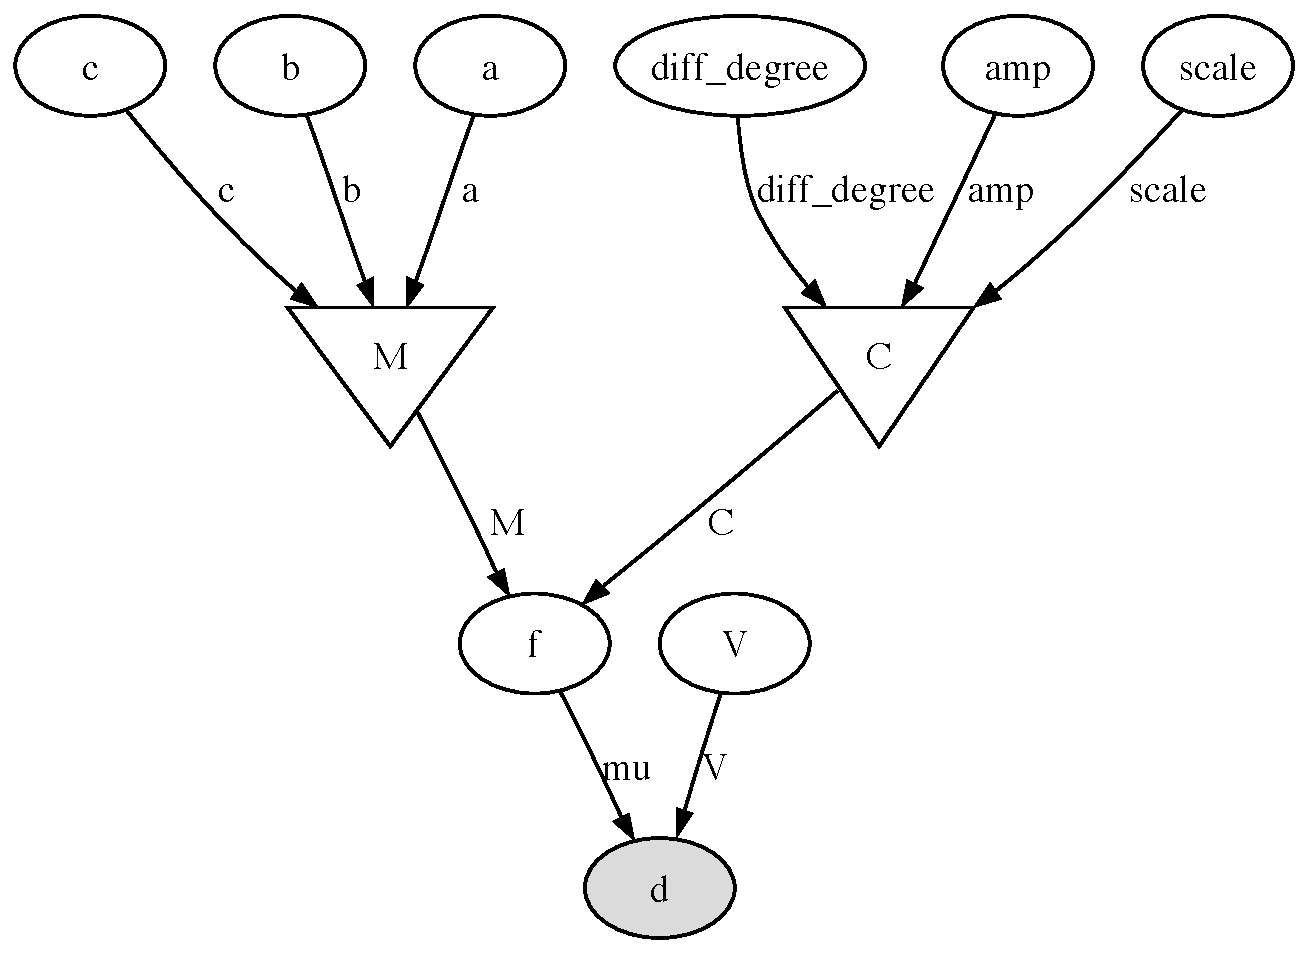
\epsfig{file=figs/unobservedModel.pdf, width=15cm}
    \caption{The \pkg{PyMC}-generated directed acyclic graph representation of the extended nonparametric regression model created by \code{pymc/examples/gp/PyMCModel.py}. Ellipses represent \code{Stochastic} objects (variables whose values are unknown even if their parents' values are known), triangles represent \code{Deterministic} objects (variables whose values can be determined if their parents' values are known), and rectangles represent \code{Stochastic} objects with the \code{isdata} flag set to \code{True} (data). Rectangles represent potentials. Arrows point from parent to child. The submodel contains the Gaussian process \code{sm\_f} and its evaluation \code{sm\_f\_eval} on input array \code{sm\_mesh}. It also contains the mean \code{sm\_M\_eval} of \code{sm\_f\_eval} and the lower-triangular Cholesky factor \code{sm\_S\_eval} of its covariance matrix, and a potential \code{sm_fr_check} that forces that covariance matrix to remain positive definite. The actual covariance evaluation \code{sm\_C\_eval} is not needed by the model, but it is exposed for use by Gibbs step methods.}
    \label{fig:unobservedModel}
\end{figure}

\begin{figure}
    \centering
        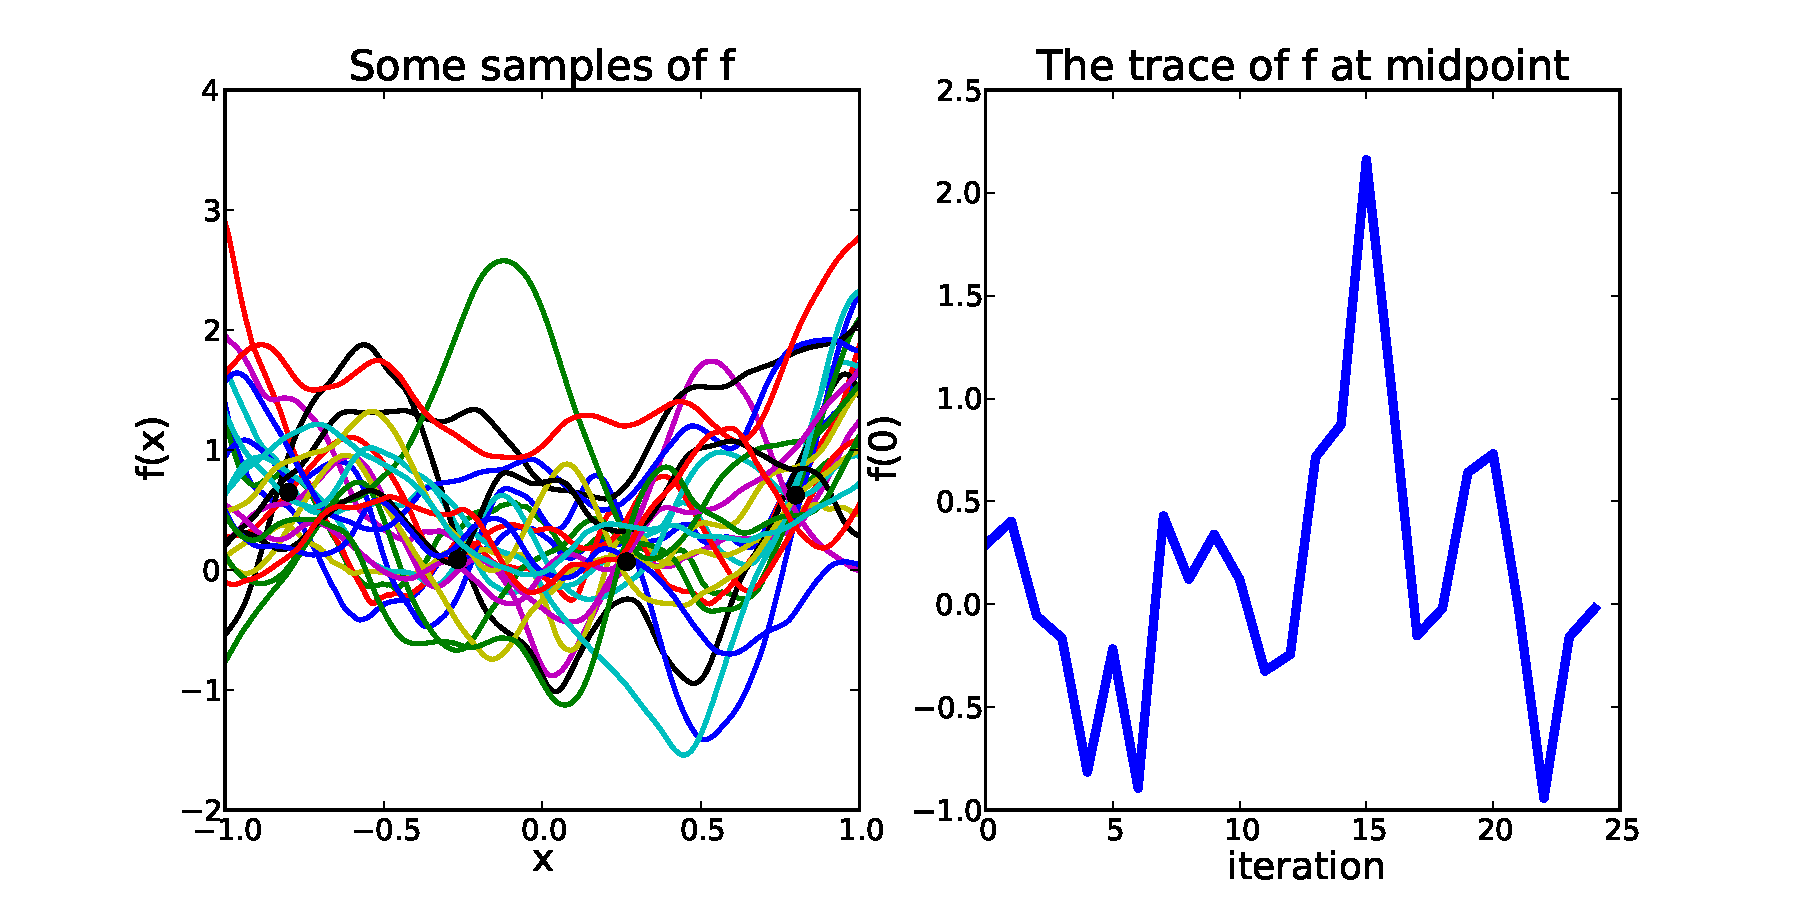
\epsfig{file=figs/gibbsSamples.pdf,width=8cm}
        % 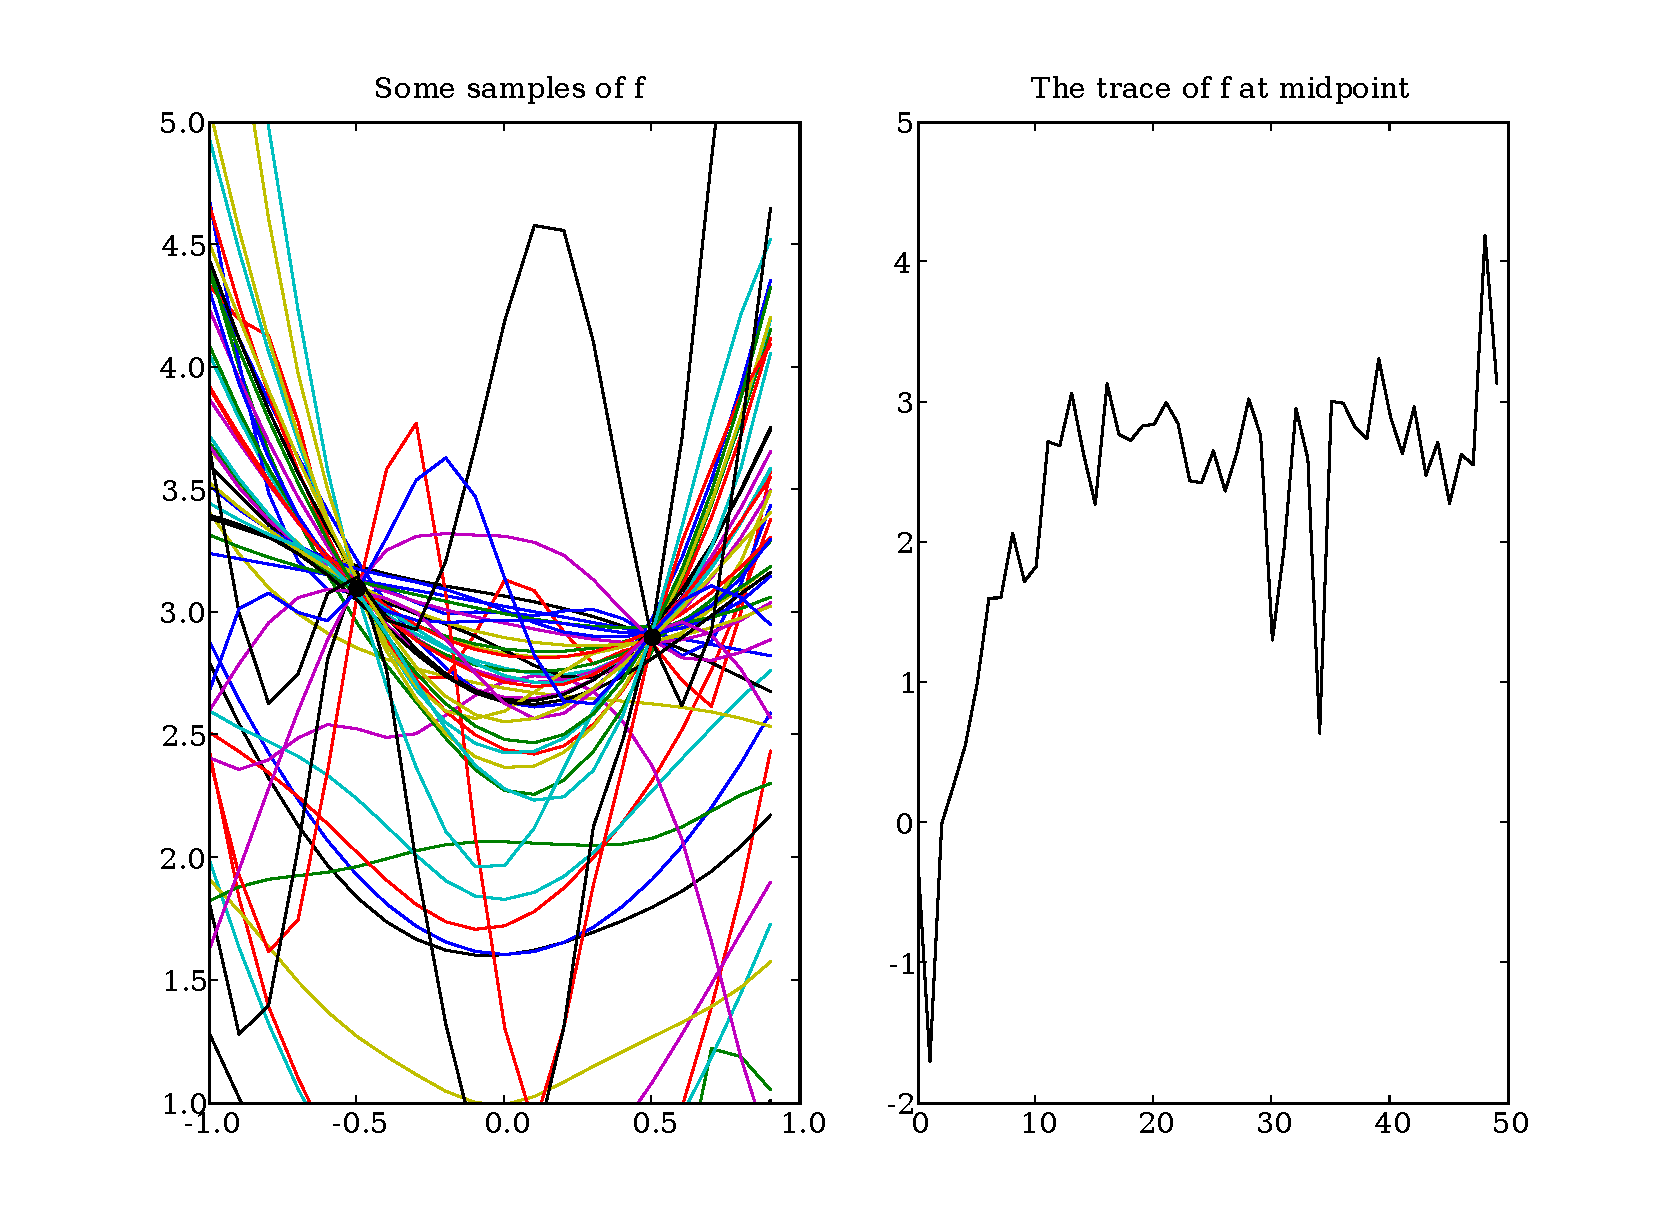
\epsfig{file=figs/metroSamples.pdf,width=10cm}
    \caption{The output of \code{pymc/examples/gp/MCMC.py}. The left-hand panel shows all the samples generated for the Gaussian process $f$, and the right-hand panel shows the trace of $f(0)$.}
    \label{fig:MCMCOutput}
\end{figure}






\section{Step methods}
% \label{sec:step-methods} 
Since $f$ has no \code{logp} attribute, the Metropolis-Hastings family of step methods \citep{pymc} cannot be used to update $f$, $f(x_*)$ or any of their mean or covariance parameters. This package uses a relatively simple work-around that will be described here. Throughout this section, the parents of $f$ are denoted $P$ and the children $K$.


\subsection{Step methods that handle parents of Gaussian processes}
If we could come up with a probability density function for $f$, the Metropolis-Hastings acceptance ratio for a proposed value $P_p$ of the parents \emph{and} a proposed value $\tilde f$ for $f$ would be:
\begin{eqnarray*}
    \frac{p(K|f_p)\ p(f_p|P_p)\ q(P)}{p(K|f)\ p(f|P)\ q(P_p)}
\end{eqnarray*}
where $q$ denotes the proposal density. Now, suppose we proposed a value for $f$ conditional on the proposed values for the parents $P$ \emph{and} conditional on $f(x_*)$. The new acceptance ratio would become
\begin{eqnarray*}
    \frac{p(K|f_p)\ p(f_p|f(x_*), P_p)\ p(f(x_*) | P_p)\ q(f_p|f(x_*),f_p, P_p)\ q(P)}{p(K|f)\ p(f|f(x_*), P)\ p(f(x_*) | P)\ q(f_p|f(x_*),f,P)\ q(P_p)}
\end{eqnarray*}
 We want to avoid computing all terms with $f$ or $f_p$ in the consequent position:
\begin{eqnarray*}
    p(f_p|f(x_*), P),\\ q(f|f(x_*),f_p,P),\\ p(f|f(x_*), P),\\ q(f_p|f(x_*),f,P_p),
\end{eqnarray*}
but all other terms are fine. We can make the problem terms cancel by choosing our proposal distribution as follows:
\begin{eqnarray*}
    q(f_p|f(x_*),f,P_p) = p(f_p|f(x_*), P).
\end{eqnarray*}
In other words, if we propose $f$ from its prior distribution conditional on $f(x_*)$ and its parents whenever we propose $f(x_*)$, we don't have to worry about computing the intractable terms. This argument can be made more rigorous by replacing $f$ with its evaluation at all the points at which we would ever want to know it.

By choosing the same proposal distribution for $\tilde f$ as above, we again avoid having to compute the intractable terms. In other words, every time a value is proposed for a \code{GP}'s parent, a value must be proposed for the \code{GP}  conditional on its value's evaluation on its mesh, and the prior probability of the \code{GP}'s children must be included in the acceptance ratio.

\smallskip
To summarize, any Metropolis-Hastings step method can handle the parents of $f$, as well as $f(x_*)$, if it proposes values for $f$ jointly with its target variable as outlined above. 

This minor alteration in jumping strategy is implemented by the function \code{wrap_metropolis_for_gp_parents}, which takes a subclass of \code{Metropolis} as an argument and returns a new step method class with altered \code{propose} and \code{reject} methods. The function automatically produces modified versions of all Metropolis step methods in \pkg{PyMC}'s step method registry (\code{Metropolis}, \code{AdaptiveMetropolis}, etc.) \citep{pymc}. The modified step methods are automatically assigned to parents of Gaussian processes.

\subsection{Choosing a mesh} 

The mesh points $x_*$ are the points where Metropolis-Hastings step methods can `grab' the value of $f$ to moderate the variance of its proposal distribution. If $x_*$ is an empty array, $f$'s value will be proposed from its prior, and rejection rates are likely to be quite large. If $x_*$ is too dense, on the other hand, computation of the log-probability of $f(x_*)$ will be expensive, as it scales as the cube of the number of points in the mesh.This continuum is illustrated in figure \ref{fig:meshpropose}. Finding the happy medium requires some experimentation.

If $f$'s children depend on its value only via its evaluation on the mesh, the likelihood terms $p(K|f_p)$ and $p(K|f)$ will cancel. In other words, if the mesh is chosen so that $p(K|f)=p(K|f(x_*))$ then the proposed value of $f$ will have no bearing on the acceptance probability of the proposed value of $f(x_*)$ or of the parents $P$. This is the situation in \code{\pkg{PyMC}Model.py}. Such a mesh choice will generally improve the acceptance rate.

\begin{figure}
    \centering
        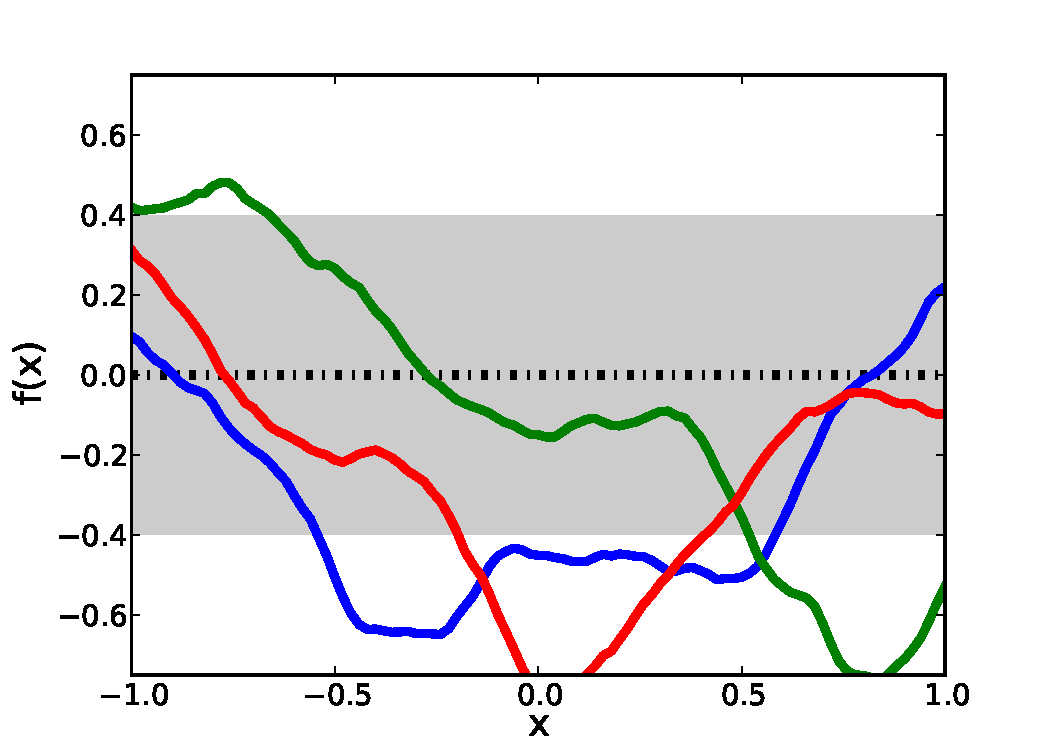
\epsfig{file=figs/nomeshpropose.pdf,width=4cm}
        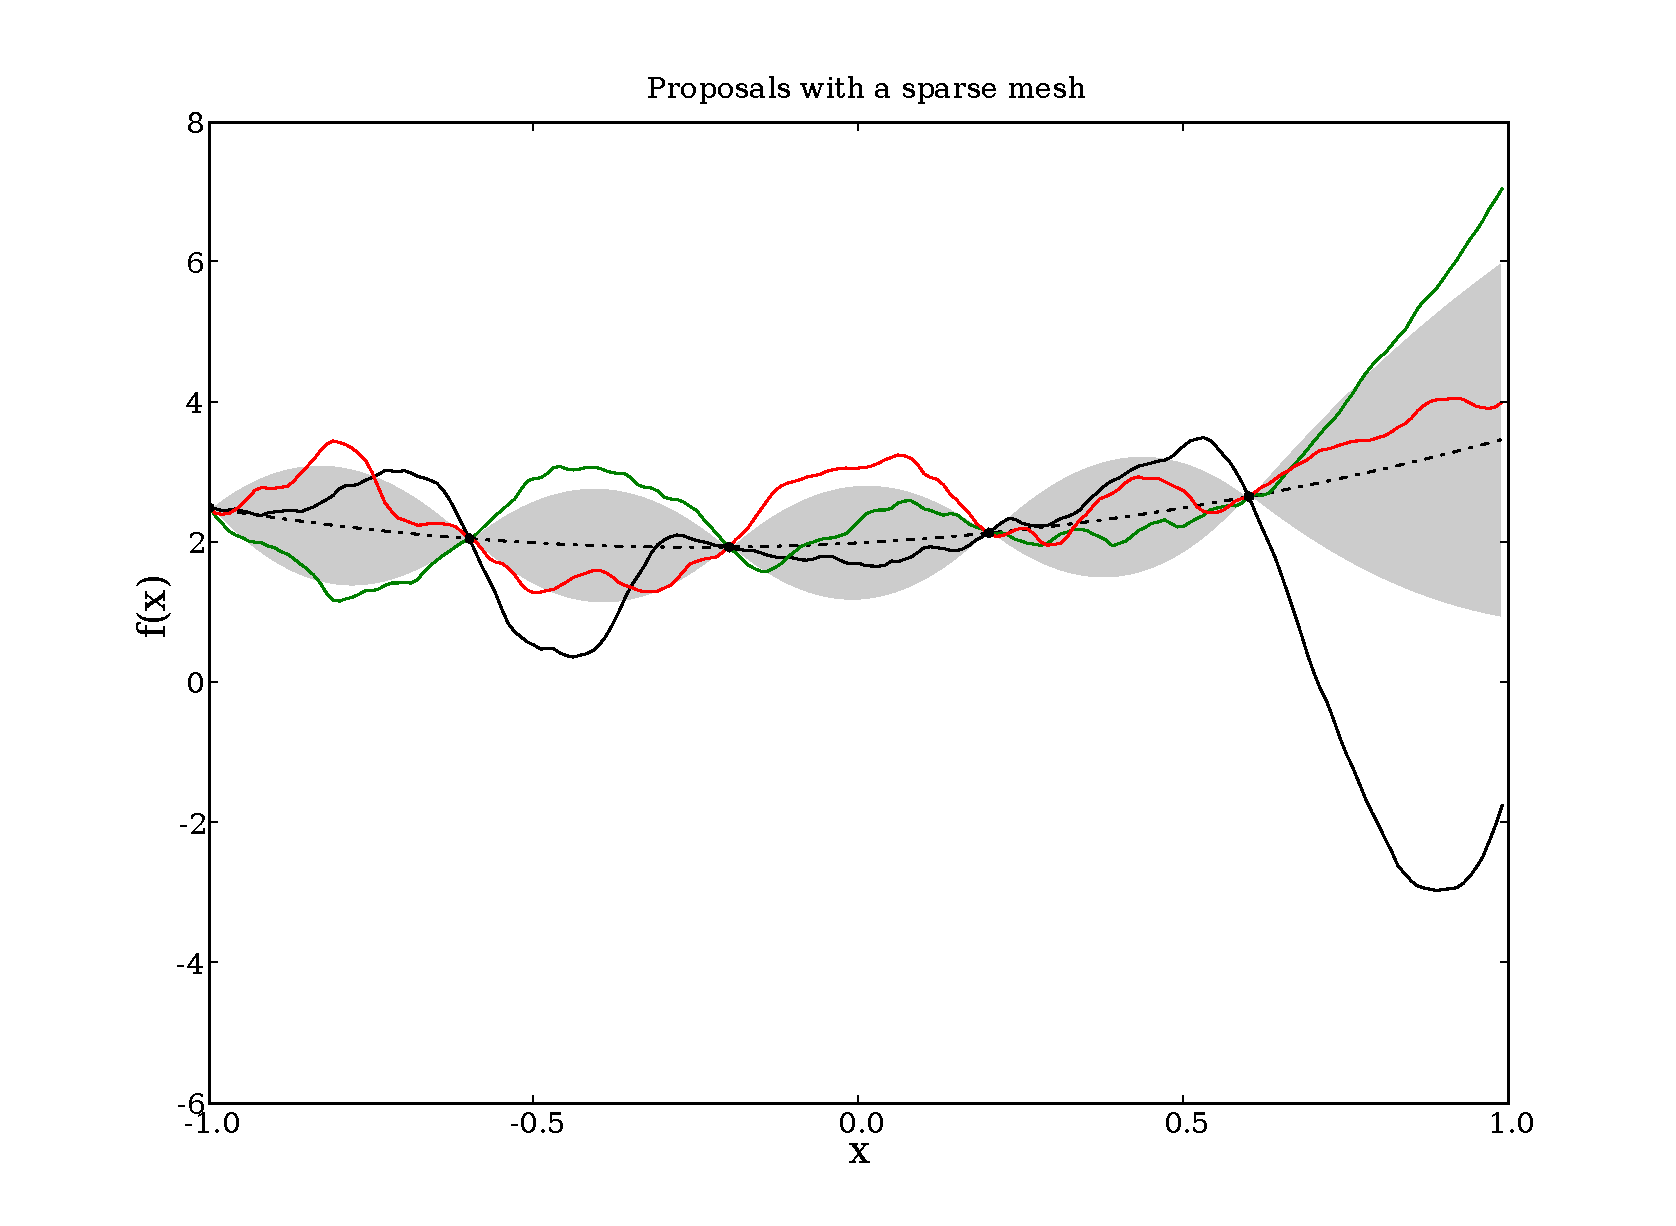
\epsfig{file=figs/lightmeshpropose.pdf,width=4cm}
        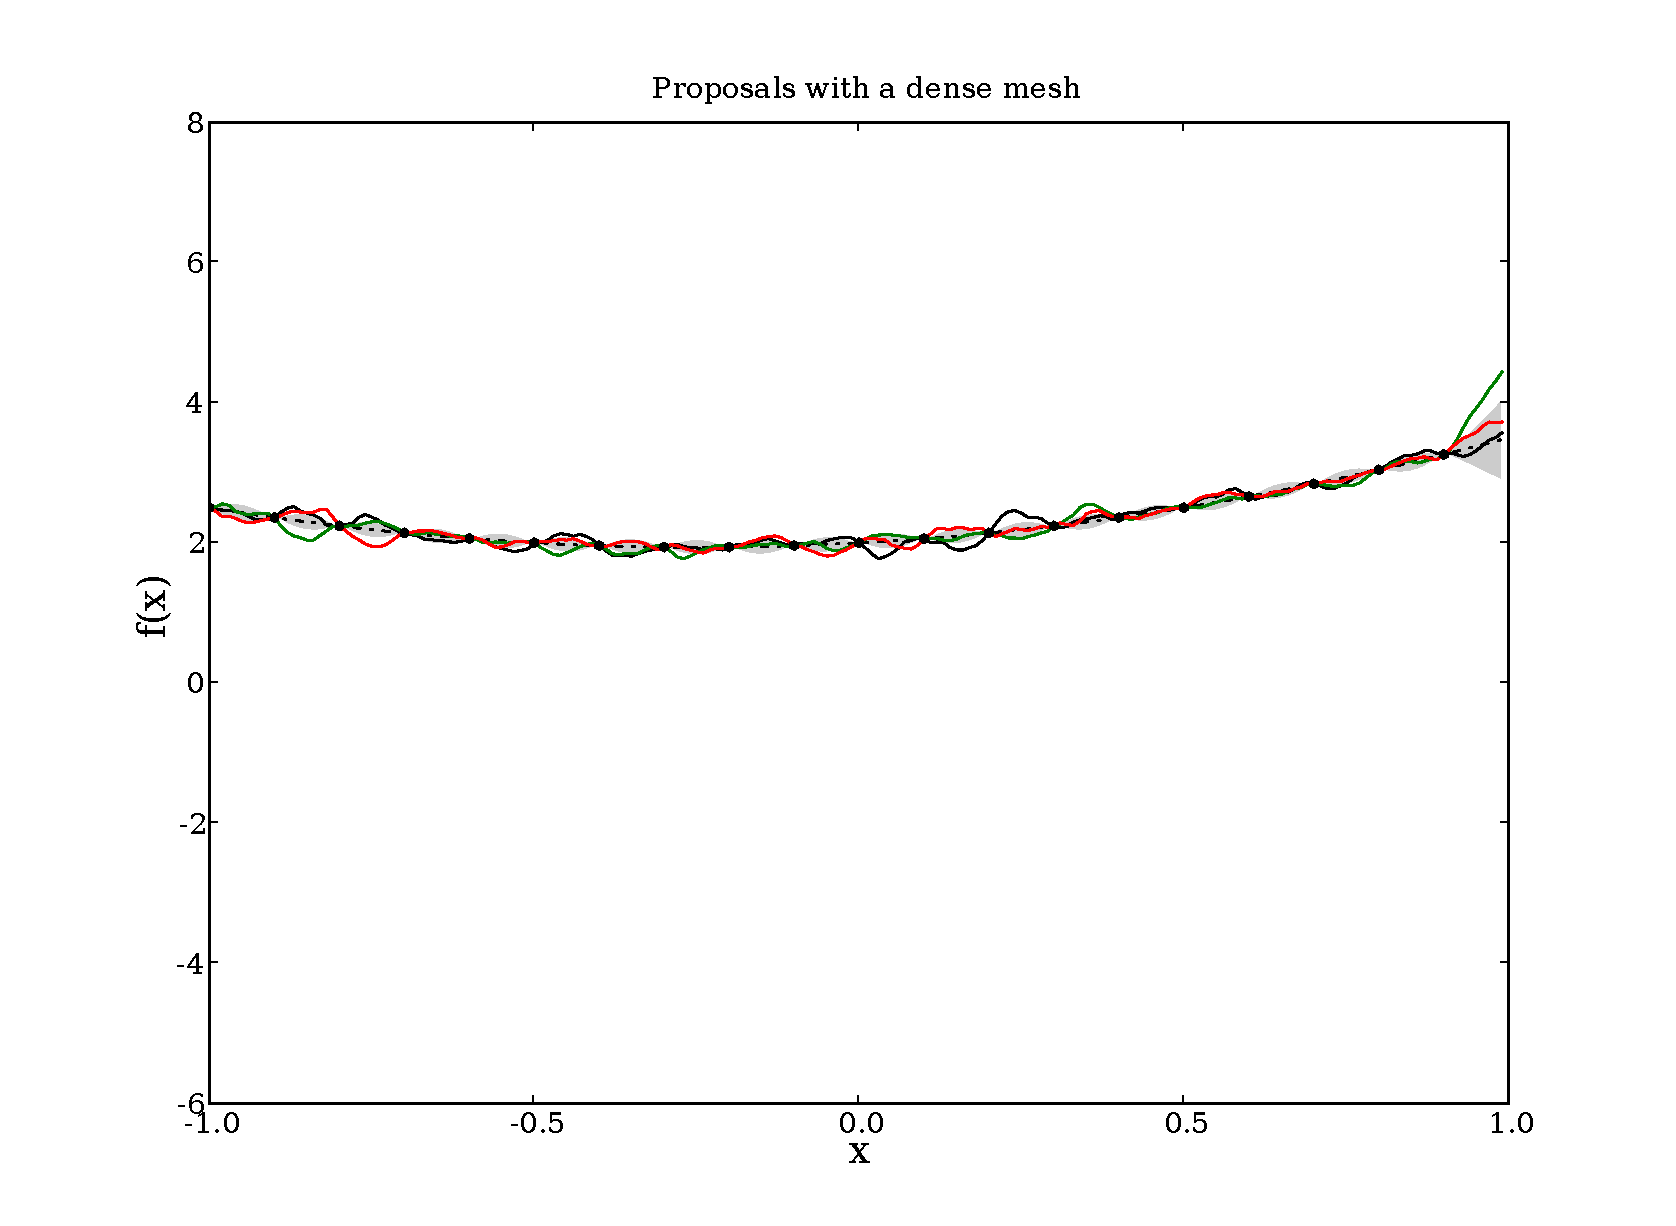
\epsfig{file=figs/densemeshpropose.pdf,width=4cm}
    \caption{Several possible proposals of $f$ (curves) given proposed values for $f(x_*)$ (heavy dots) with no mesh (top), a sparse mesh (middle), and a dense mesh (bottom). Proposal distributions' envelopes are shown as shaded regions, with means shown as broken lines. With no mesh, $f$ is proposed from its prior and the acceptance rate will be very low. A denser mesh permits a high degree of control over $f$, but computing the log-probability will be more expensive.}
    \label{fig:meshpropose}
\end{figure}

\subsection{Gibbs steps} 
If all of $f$'s children, $K$, depend on it as follows:
\begin{eqnarray*}
    K_i|f \stackrel{\textup{\tiny ind}}{\sim} \textup{Normal}(f(x_{*i}),V_i)
\end{eqnarray*}
then $f(x_*)$ can be handled by the \code{GPEvaluationGibbs} step method. This step method is used in \code{MCMC.py}:
\begin{CodeChunk}
\begin{CodeInput}
GPSampler.use_step_method(gp.GPEvaluationGibbs, GPSampler.submod, \
    GPSampler.V, GPSampler.d)
\end{CodeInput}
\end{CodeChunk}
The initialization arguments are the Gaussian process submodel that contains $f$, the observation variance of $f$'s children, and the children, in this case the vector-valued normal variable $d$. 

\code{GPEvaluationGibbs} covers the standard submodel encountered in geostatistics, but there are many conjugate situations to which it does not apply. If necessary, special step methods can be written to handle these situations. If \code{GPEvaluationGibbs} is not assigned manually, $f(x_*)$ will generally be handled by a wrapped version of \code{AdaptiveMetropolis} \citep{pymc}.





\section{Geostatistical example}\label{sub:geostat}
\begin{figure}
    \centering
        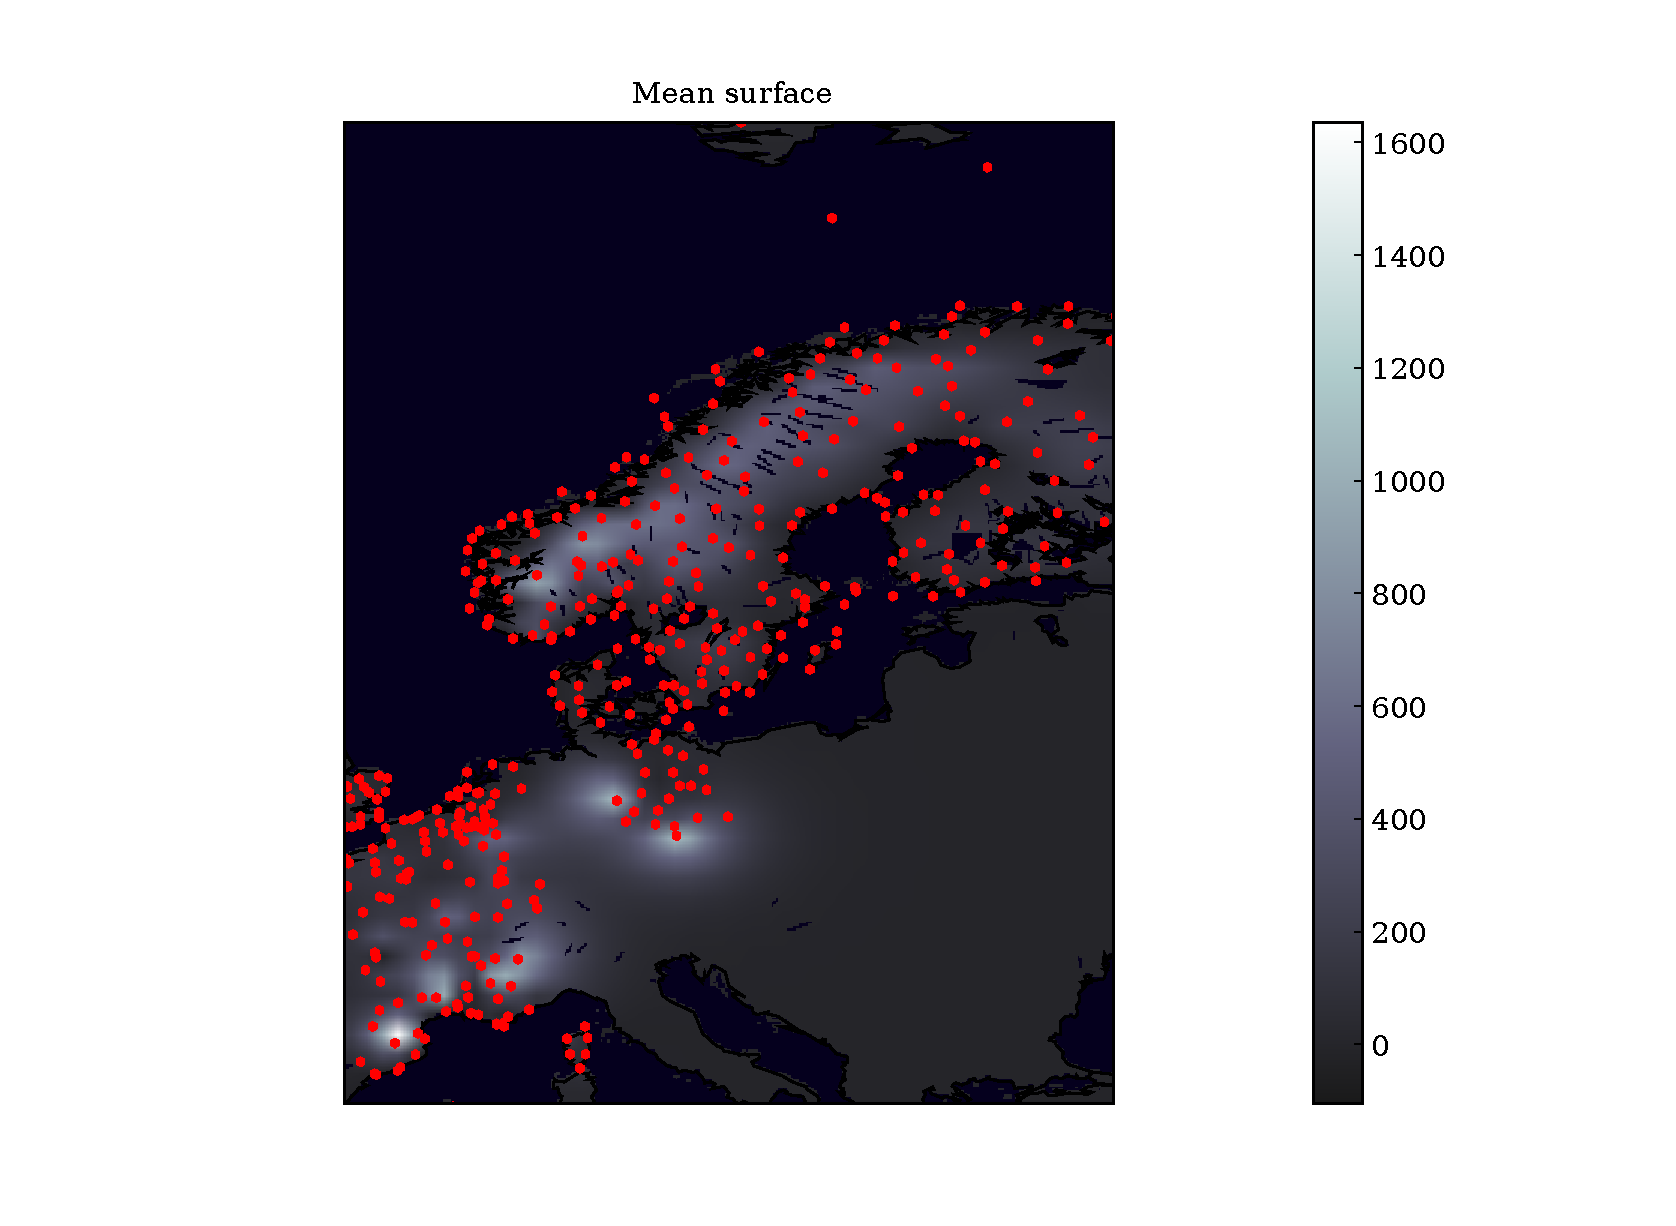
\epsfig{file=figs/elevmean.pdf, width=5cm}
        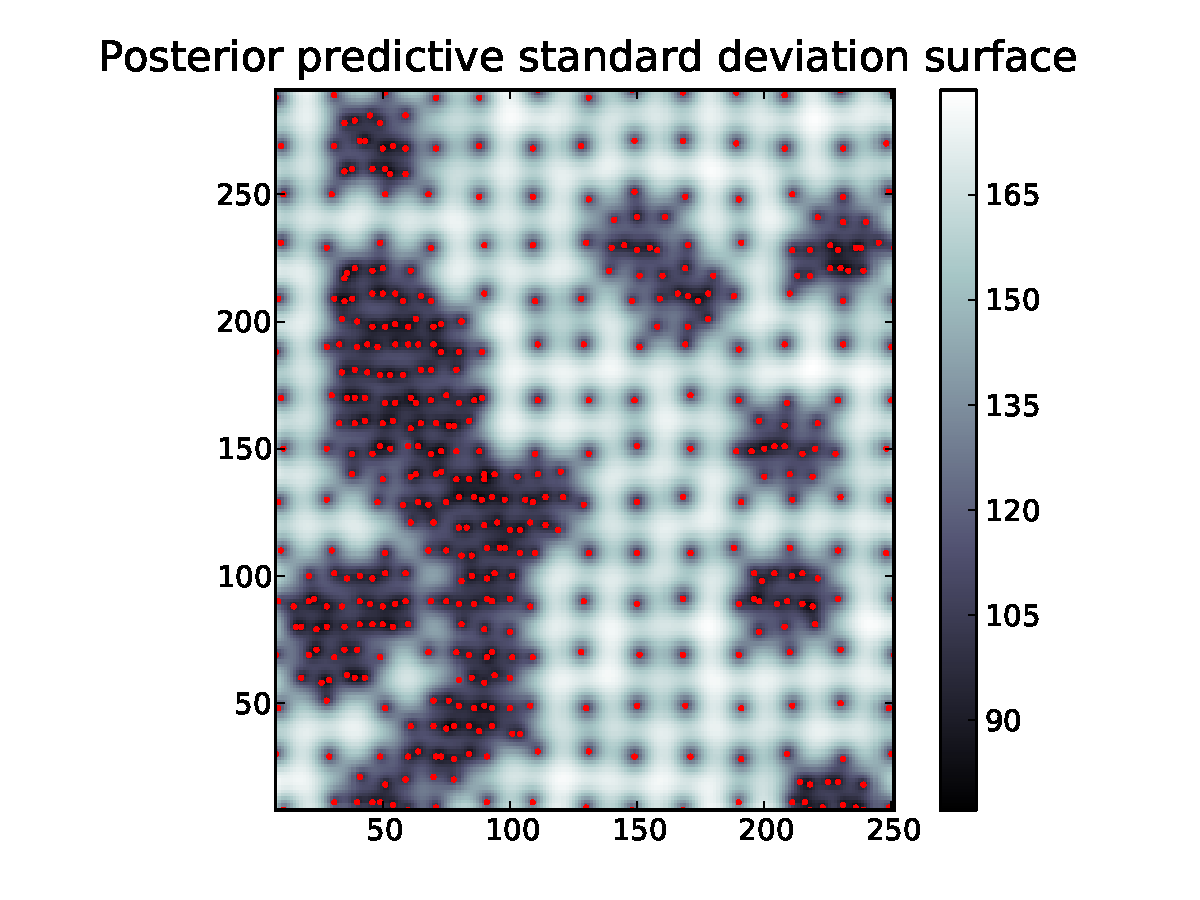
\epsfig{file=figs/elevvar.pdf, width=5cm}
    \caption{The posterior mean and variance surfaces for the $v$ variable of the Walker lake example. The posterior variance is relatively small in the neighborhood of observations, but large in regions where no observations were made.}
    \label{fig:walker}
\end{figure}
\begin{figure}
    \centering
        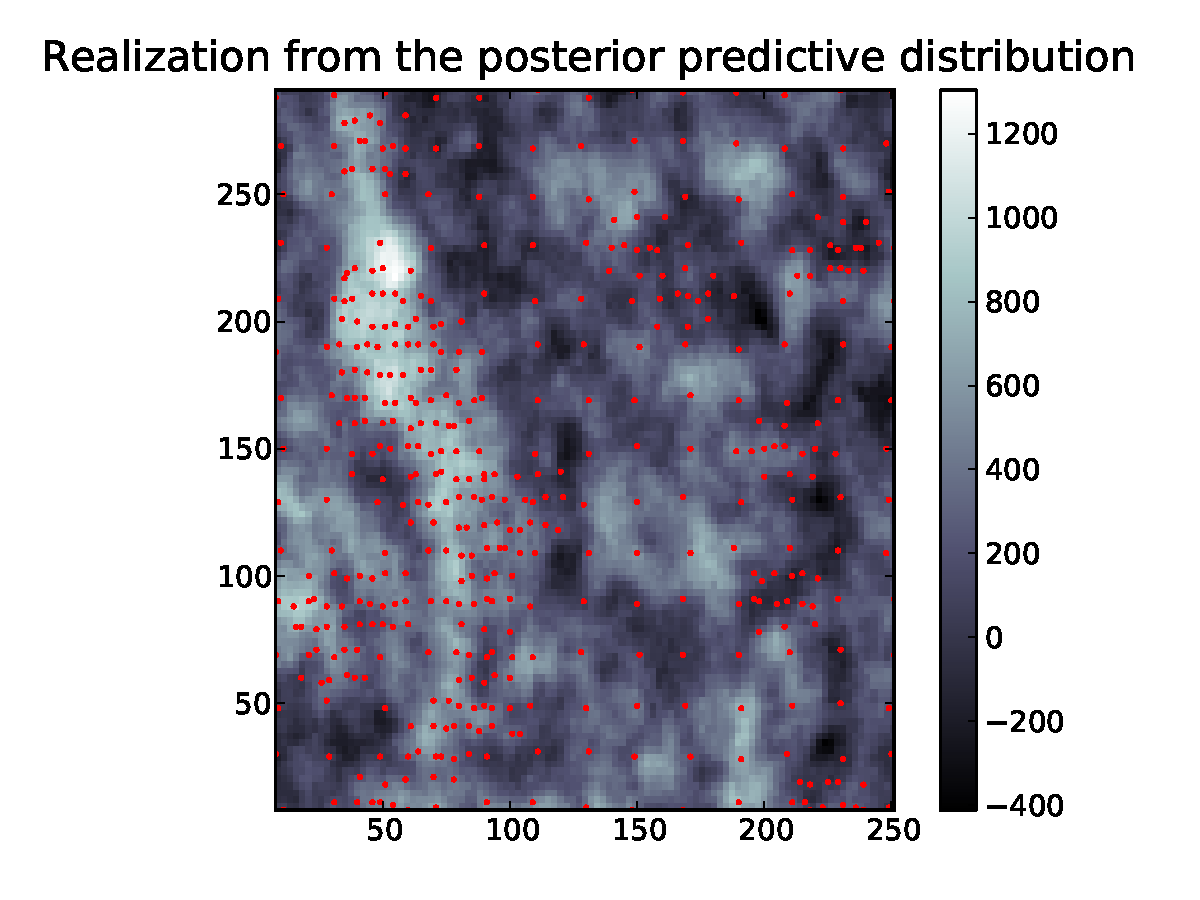
\epsfig{file=figs/elevdraw0.pdf, width=5cm}
        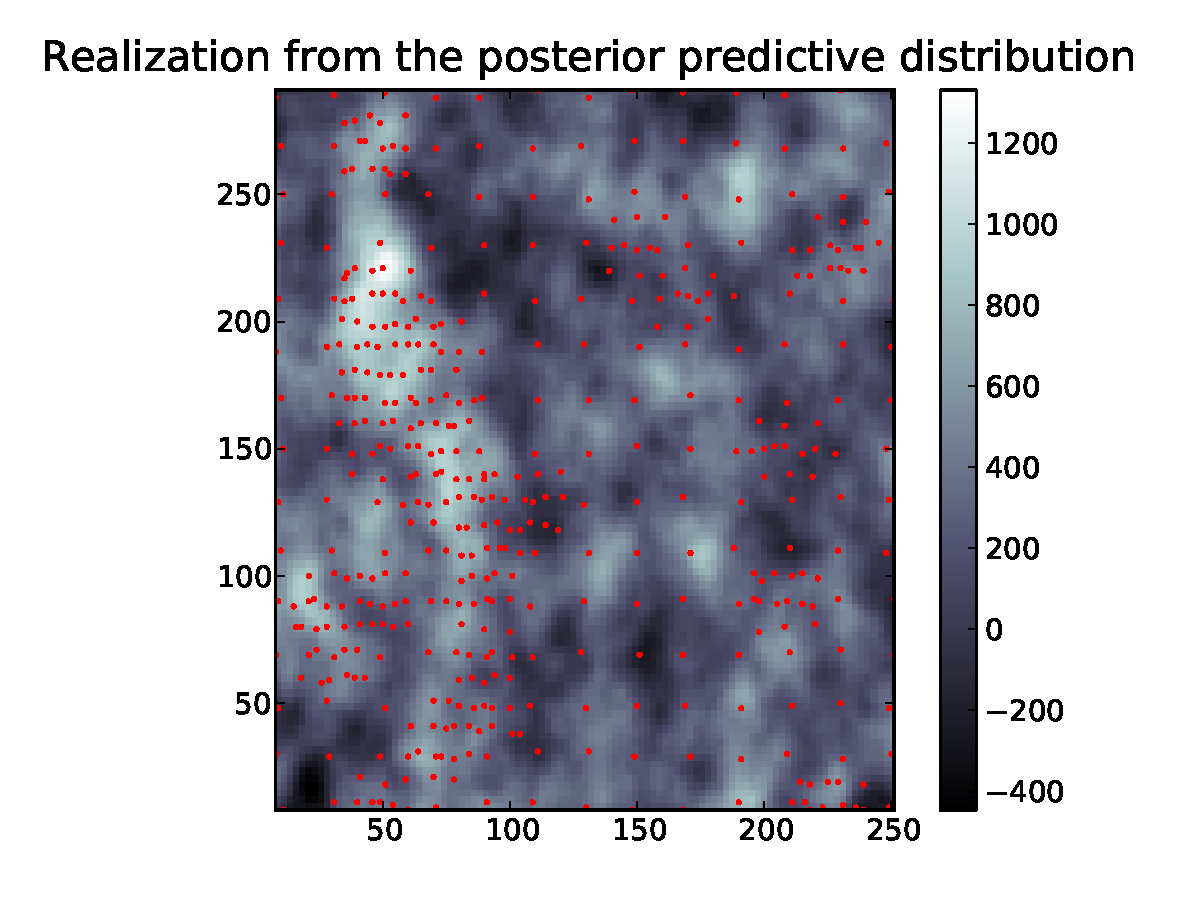
\epsfig{file=figs/elevdraw1.pdf, width=5cm}
    \caption{Two realizations from the posterior distribution of the $v$ surface for the Walker Lake example. Elevation is measured in meters.}
    \label{fig:walkerreal}
\end{figure}
Bayesian geostatistics is demonstrated in the folder \code{pymc/examples/gp/more_examples/Geostatistics}. File \code{getdata.py} downloads the Walker Lake dataset of Isaaks and Srivastava \citep{isaaks} from the internet and manipulates the $x$ and $y$ coordinates into the array format described in section \ref{sec:highdim}. File \code{model.py} contains the geostatistical model specification, which is

\begin{eqnarray*}
    d|f \sim \textup{Normal}(f(x),V)\\
    f|M,C \sim \textup{GP}(M,C) \\
    M:x\rightarrow m\\
    C:x,y,\mathtt{amp},\mathtt{scale},\mathtt{diff\_degree}\rightarrow \mathtt{matern.euclidean}(x,y;\mathtt{amp},\mathtt{scale},\mathtt{diff\_degree})\\
    p(m)\propto 1\\
    \mathtt{amp}\sim \textup{Exponential}(7e-5) \\
    \mathtt{scale}\sim \textup{Exponential}(4e-3) \\
    \mathtt{diff\_degree}\sim \textup{Uniform}(.5,2)\\ 
    V\sim \textup{Exponential}(5e-9)\\
\end{eqnarray*}

File \code{mcmc.py} fits the model and produces output maps.  The output of \code{mcmc.py} is shown in figures \ref{fig:walker} and \ref{fig:walkerreal}. Figure \ref{fig:walker} shows the posterior mean and variance of the $v$ variable of the dataset, which is a function of elevation (see \cite{isaaks}, appendix A).